\documentclass[11pt,a4paper]{article}
\usepackage{fullpage}
\usepackage[T1]{fontenc} 
\usepackage[utf8]{inputenc}
\usepackage{amsmath}
\usepackage{amssymb}
\usepackage{float}
\usepackage{tabularx}
\usepackage{multirow}
\usepackage{graphicx}
\usepackage{geometry}
\usepackage[table,dvipsnames]{xcolor}
\usepackage[hidelinks]{hyperref}
\usepackage[polish]{babel}
\usepackage{menukeys}
\usepackage{subcaption}

\setlength{\parindent}{0cm}
\setlength{\parskip}{2mm}
\newcolumntype{Y}{>{\centering\arraybackslash}X}
\DeclareMathOperator{\sgn}{sgn}

\begin{document}

\title{Rozpoznawanie człowieka metodami biometrii \\
\Large{
    Projekt 1. --- Rozpoznawanie tęczówki \\
    Raport
}}
\author{Bartłomiej Dach}
\maketitle

Poniższy dokument stanowi sprawozdanie z~implementacji aplikacji dokonującej rozpoznawania człowieka na~podstawie tęczówki wysegmentowanej ze~zdjęć oczu.
W~dokumencie opisano zastosowane metody segmentacji, przetwarzania i~porównywania obrazów tęczówek oraz~zawarto wyniki działania dla~wybranych przykładowych obrazów wejściowych.

\section{Wstęp}

Analiza tęczówki jest jedną z~najpopularniejszych metod identyfikacji tożsamości człowieka znanych biometrii.
Główną przyczyną popularności tej cechy jest jej przystosowanie do~potrzeb identyfikacji --- tęczówka jest częścią oka, które jest chroniony przed~zniszczeniem przez~rogówkę i~powieki.
Dodatkowo tęczówka ma~teksturę z~dużą liczbą szczegółów, która powoduje, że z~dużym prawdopodobieństwem można stwierdzić jej~unikalność.
Z~tego powodu, pomimo tego, że~pozyskanie dobrego obrazu wymaga kooperacji osoby rozpoznawanej poprzez~zbliżenie oka do~aparatu, tęczówka jest jedną z~najlepszych znanych metod rozpoznawania.

W~ramach projektu zaimplementowano metodę identyfikacji na~podstawie tęczówki opracowaną przez~Daugmana~\cite{daugman2004, slot2008}.
W~wyniku tej metody obrazy tęczówek są~konwertowane na~binarny 2048-bitowy kod tęczówki.
Szczegółowy opis metody znajduje~się w~sekcji~\ref{sec:method}.

\section{Opis aplikacji}

W~ramach projektu stworzony został program okienkowy umożliwiający gromadzenie i~porównywanie obrazów ludzkich oczu.
Program został napisany w~języku Java w~wersji~8.

Do~stworzenia interfejsu użytkownika została wybrana biblioteka JavaFX \cite{javafx}.
Główną motywacją wyboru tej biblioteki były:
\begin{itemize}
    \item zgodność z~wieloma platformami (Windows, Linux, Mac),
    \item wbudowane w~bibliotekę klasy pozwalające na~edycję bitmap poprzez zmianę kolorów pojedynczych pikseli, co~umożliwia samodzielną realizację filtrów, na~których oparta jest operacja segmentacji oraz~implementację algorytmu rozpoznawania.
\end{itemize}

\begin{figure}
    \centering
    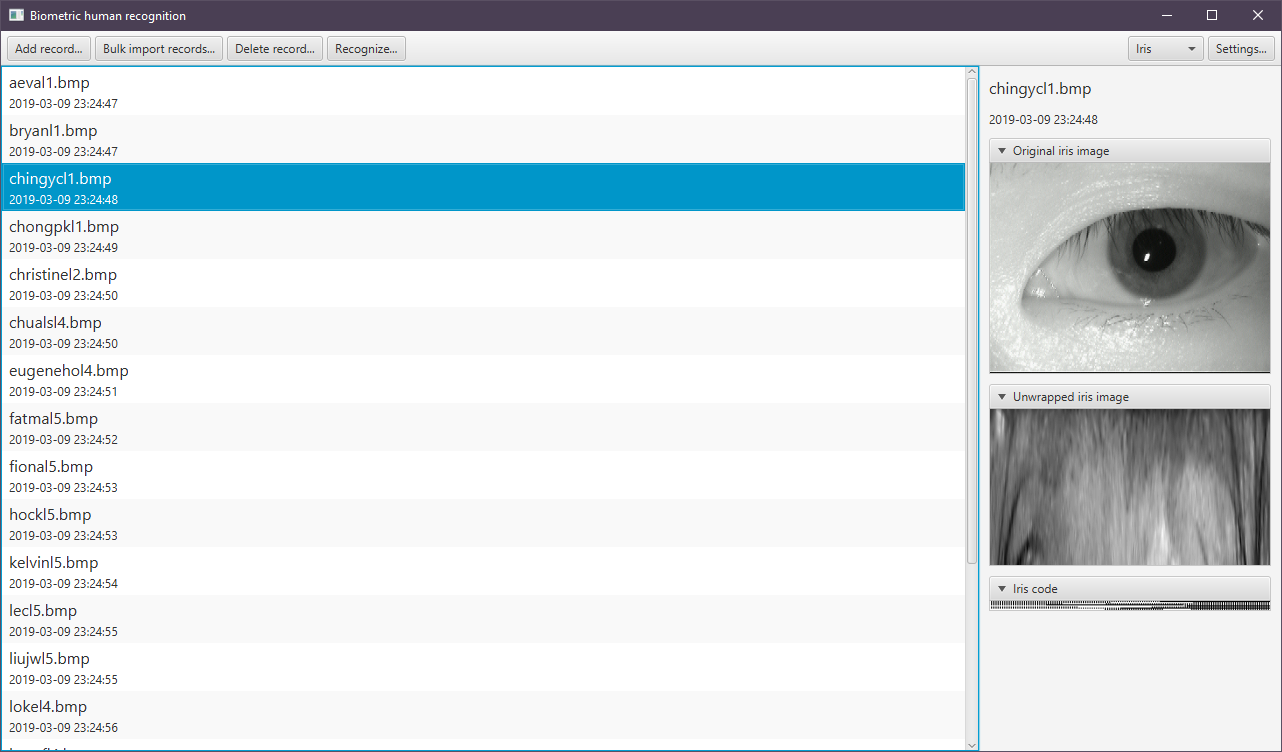
\includegraphics[width=\textwidth]{res/img/main-window.PNG}
    \caption{Główne okno zaimplementowanej aplikacji.}
    \label{fig:main-window}
\end{figure}

\begin{figure}
    \centering
    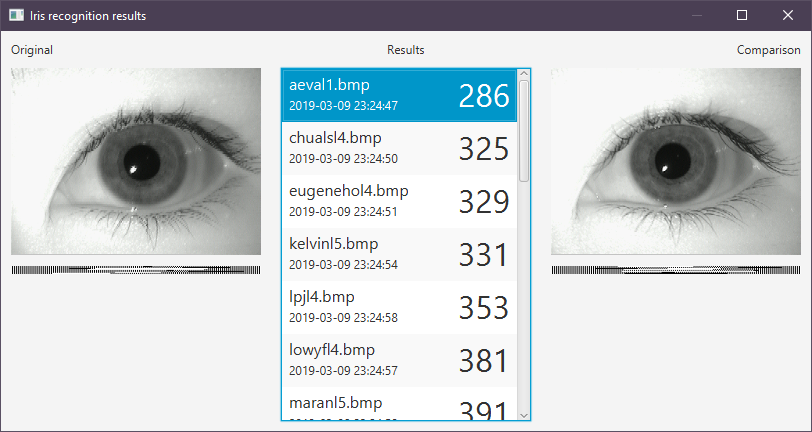
\includegraphics[width=\textwidth]{res/img/recognition-results.PNG}
    \caption{Widok z~wynikami rozpoznawania.
    Możliwe jest porównanie wizualne rozpoznawanego obrazu z~tymi umieszczonymi w~bazie.}
    \label{fig:recognition-results}
\end{figure}

\subsection{Instrukcja obsługi}

Po~uruchomieniu aplikacji widocznej jest główne okno, przedstawione na~rysunku~\ref{fig:main-window}.
Aplikacja pozwala zarządzać bazą zgromadzonych obrazów tęczówek i~rozpoznawać nowe~obrazy z~tęczówkami w~bazie.
Na~pasku narzędziowym udostępnione~są następujące akcje:

\begin{itemize}
    \item Przycisk \keys{Add record...} pozwala na~dodanie nowego rekordu ze~zdjęciem tęczówki do~bazy.
    \item Przycisk \keys{Bulk import records...} pozwala na~dodanie wielu nowych rekordów za~jednym razem poprzez wybranie grupy zdjęć tęczówek do~zaimportowania.
    \item Przycisk \keys{Delete record...} pozwala na~usunięcie zaznaczonego rekordu z~bazy.
    \item Przycisk \keys{Recognize...} pozwala na~porównanie wybranego zdjęcia ze~zdjęciami zgromadzonymi w~bazie i~wyświetla wyniki porównania.
    Wyniki są~posortowane względem stopnia podobieństwa do~referencyjnego obrazu.
    Przykład widoku z~wynikami widoczny jest na~rysunku~\ref{fig:recognition-results}.
    \item Przycisk \keys{Settings...} pozwala na~zmianę ustawień rozpoznawania.
    W~przypadku tęczówki jedynym parametrem konfiguracyjnym jest częstotliwość falek~Gabora używanych podczas~transformaty falkowej opisanej w~podsekcji~\ref{subsec:recognition}.
    Zmiana częstotliwości powoduje ponowne obliczenie kodów dla~wszystkich tęczówek w~bazie.
\end{itemize}

\section{Opis metody}
\label{sec:method}

W~procesie rozpoznawania można wyróżnić trzy główne etapy:
\begin{enumerate}
    \item segmentacja obrazu w~celu znalezienia granic tęczówki na~zebranym obrazie,
    \item właściwe przetwarzanie rozwiniętego obrazu tęczówki w~celu wyznaczenia kodu tęczówki,
    \item porównywanie obliczonych kodów tęczówek w~celu wyznaczenia stopnia podobieństwa dwóch obrazów, umożliwiającego identyfikację osoby na~obrazie.
\end{enumerate}
W~ogólności algorytm rozpoznawania wykorzystuje: filtry liniowe i~nieliniowe, interpolację biliniową, dyskretną transformatę falkową oraz~odległość Hamminga.

\subsection{Segmentacja obrazu}

Celem pierwszej fazy jest wyznaczenie obszaru obrazu, na~którym znajduje się tęczówka.
Metoda została przeniesiona bezpośrednio z~projektu opracowanego na~potrzeby przedmiotu ,,Analiza i~przetwarzanie obrazów biometrycznych''.

Zaimplementowana metoda segmentacji należy do~grona metod proceduralnych, tj.~stosuje ściśle określoną listę operacji i~nie stosuje metod optymalizacyjnych lub~stochastycznych.
Kolejne kroki przetwarzania wejściowego obrazu w~celu lokalizacji tęczówki ilustruje rysunek~\ref{fig:block-diagram}.
Opis~poszczególnych operacji znajduje~się w~poszczególnych częściach tego~rozdziału.

Ogólnie mówiąc, proces lokalizacji tęczówki opiera~się na~uprzednim zlokalizowaniu źrenicy.
Przy~lokalizacji przyjęto następujące założenia:
\begin{itemize}
    \item Źrenica jest największym ciemnym obszarem na~obrazie wejściowym.
    \item Źrenicę i~tęczówkę można uznać za~okręgi koncentryczne (tj. środek źrenicy jest również środkiem tęczówki).
\end{itemize}
Z~tego względu w~algorytmie stosowane~są dwa łańcuchy operacji, których wyniki używane są do~geometrycznej lokalizacji środka źrenicy oraz promieni: wewnętrznego i~zewnętrznego źrenicy.

\paragraph{Rozciągnięcie histogramu.}
Na~początku algorytmu wykonywane jest rozciągnięcie histogramu poszczególnych kanałów obrazu zgodnie ze~wzorem
$$ I_o = \frac{I_i - I_{\min}}{I_{\max} - I_{\min}} $$
Celem tej~operacji jest maksymalizacja dynamiki obrazów bez~utraty danych.
Po~jej wykonaniu na~każdym kanale jasność wszystkich pikseli znajduje~się dokładnie w~przedziale $[0, 255]$ (zakładając 8-bitową głębię koloru).
Jest to~istotne szczególnie na~etapie progowania, gdzie~błędy przybliżeń progu mogą mieć znaczące znaczenie na~końcowy wynik.

\paragraph{Filtr gaussowski.}
Po~rozciągnięciu histogramu stosowany jest splotowy filtr gaussowski o~rozmiarze elementu~$3 \times 3$, określonego macierzą
$$ F_g = \begin{bmatrix}
    1 & a & 1 \\
    a & a^2 & a \\
    1 & a & 1
\end{bmatrix} $$
gdzie $a > 1$ stanowi parametr filtra.

Filtr gaussowski jest filtrem dolnoprzepustowym, którego zastosowanie powoduje wygładzenie obrazu.
Celem tej operacji w~łańcuchu jest zamaskowanie szczegółów nieistotnych dla~procesu segmentacji, takich, jak m.in.~ziarno czy~pomijalne przebarwienia małych fragmentów obrazu.

Im większa wartość parametru~$a$, tym mniej zauważalny jest efekt rozmycia.
W~przypadku źrenicy, stosowany jest parametr $a = 1.5$, zaś dla~tęczówki --- $a = 1.8$.
Uzasadnieniem tej rozbieżności jest fakt, że na~ogół zewnętrzny brzeg tęczówki jest mniej ostry niż~brzeg źrenicy, zatem aby zapobiec przekłamaniom przy~pomiarze zewnętrznego promienia, stosowane jest mniejsze rozmycie.

\paragraph{Konwersja do~skali szarości.}
Na~podstawie rozmytego obrazu kolorowego stosowane jest przejście do~skali szarości wg~wzoru
$$ I_o = r \cdot I_r + g \cdot I_g + b \cdot I_b $$
gdzie $I_r, I_g, I_b$ reprezentują jasności pikseli na~kanałach odpowiednio: czerwonym, zielonym i~niebieskim, zaś~$r, g, b$ są~współczynnikami konwersji.
Zarówno dla~tęczówki, jak i~dla~źrenicy przyjęto wspólne wartości
$$ r = 0.299, \qquad g = 0.587, \qquad b = 0.114 $$
odwzorowujące luminancję pikseli w~modelu kolorów YCbCr.

\paragraph{Progowanie.}
Po~konwersji do~skali szarości następuje przejście do~obrazu binarnego poprzez wykonanie operacji progowania zgodnie ze~wzorem
$$ I_o = \begin{cases}
    0, & I_i < t \\
    1, & I_i \geq t
\end{cases} $$
gdzie próg $t$ wyznaczany jest na~podstawie poziomów szarości całego obrazu ze~wzoru
$$ t = \frac{1}{d} \sum_{i = 0}^{W - 1} \sum_{j = 0}^{H - 1} I_{ij} $$
w~którym $W, H$ oznaczają wymiary obrazu (odpowiednio szerokość i~wysokość), zaś~$d$ jest nowym parametrem progowania, określającym stosunek przyjętego progu do~średniej jasności obrazu.

Im większa wartość $d$, tym mniejszy przyjęty próg.
Z~tego względu przyjęto wartość $d_p = 5.5$ dla~lokalizacji źrenicy i~$d_i = 1.4$ dla~dopasowania tęczówki.

\paragraph{Operacje morfologiczne.}
Po~progowaniu do~obrazów wynikowych stosowane są~operacje morfologiczne.
Dwoma podstawowymi operacjami morfologicznymi są: dylacja (rozszerzenie) i~erozja.
Obie operacje używają tzw.~elementu strukturalnego, który można przedstawić jako~macierz.
\begin{itemize}
    \item Operacja dylacji obrazu binarnego polega na~rozszerzeniu obiektu (tutaj zakładamy, że obiekt jest czarny na~białym tle).
    Dla~każdego czarnego piksela następuje translacja elementu strukturalnego tak, aby~jego środek znajdował~się w~danym pikselu, po~czym przesunięty element strukturalny dodawany jest do~obrazu wynikowego.
    \item Operacja erozji powoduje zwężenie obiektu.
    Dla~każdego piksela obrazu wyjściowego rozważany jest element strukturalny przesunięty tak, aby~jego środek leżał na~danym pikselu.
    Jeśli w~obrazie wejściowym przesunięty element strukturalny leży na~samych czarnych pikselach, wtedy wyjściowy piksel też ma~kolor czarny; w~przeciwnym wypadku przyjmowany jest kolor biały.
\end{itemize}
W~przypadku zaimplementowanej metody rozważane~są tylko pełne, kwadratowe elementy strukturalne o~ustalonym rozmiarze $k \times k$.

Złożenie operacji dylacji i~erozji pozwala na~zdefiniowanie dwóch innych operacji morfologicznych, w~zależności od~przyjętej kolejności:
\begin{itemize}
    \item Na~operację zamknięcia obrazu składa~się kolejno: dylacja i~erozja.
    Operacja wypełnia luki w~transformowanym obrazie.

    W~opisywanej metodzie zamknięcie stosowane jest pod~detekcję zewnętrznego konturu tęczówki.
    Wybór ten motywowany jest tym, że~tęczówka jest stosunkowo wielobarwna, co~może zakłócić wynik progowania i~wpłynąć negatywnie na~dopasowanie zewnętrznego promienia tęczówki.
    \item Na~operację otwarcia składa~się natomiast kolejno: erozja i~dylacja.
    Operacja usuwa drobny szum i~zakłócenia z~pierwszego planu obrazu.

    Otwarcie stosowane jest do~detekcji źrenicy.
    Do~wyznaczenia lokalizacji źrenicy stosowane są~projekcje --- szum na~obrazie może zakłócić wyznaczone projekcje, tym samym utrudniając zlokalizowanie źrenicy.
    Zastosowanie otwarcia pozwala wyeliminować niepożądane elementy pierwszego planu.
\end{itemize}

\paragraph{Określenie granic źrenicy.}

Po~wykonaniu jednego łańcucha operacji przeznaczonego dla~źrenicy następuje jej lokalizacja.
Odbywa~się ona przy~pomocy projekcji.

Projekcja obrazu binarnego względem jednej z~osi obrazu określa liczbę pikseli czarnych (pierwszego planu) dla~poszczególnych współrzędnych wzdłuż wybranej osi.
Zakładając, że~po~progowaniu i~operacjach morfologicznych na~obrazie zostanie sama~źrenica, to~maksimum na~projekcjach względem obu~osi powinno wskazywać na~środek źrenicy.

Na~niektórych obrazach zdarza~się jednak, że~na~źrenicy znajdują~się refleksy, np.~od~lampy błyskowej urządzenia rejestrującego.
Może to~powodować przesunięcie środka źrenicy, co~źle wpłynie na~detekcję tęczówki z~racji przyjętego założenia o~jej koncentryczności ze~źrenicą.
Z~tego względu punkt wynikający z~projekcji nie~jest uznawany automatycznie za~środek źrenicy, lecz jako~punkt startowy do~dalszych operacji.

Algorytm znajduje granice źrenicy poprzez przeszukiwanie sąsiedztwa punktu startowego.
Przeszukiwanie to~przypomina algorytm wypełniania kubełkowego (ang. \emph{flood-fill}).
Na~tej podstawie możliwe jest wyznaczenie prostokąta ograniczającego (ang. \emph{bounding box}) źrenicy, skąd stosunkowo łatwo można wyznaczyć środek i~promień źrenicy.
Środek źrenicy to~środek prostokąta, natomiast za~promień źrenicy przyjmowana jest średnia z~szerokości i~wysokości prostokąta.

\paragraph{Wyznaczenie promienia tęczówki.}
Zewnętrzny promień tęczówki obliczany jest z~drugiego zbinaryzowanego obrazu z~użyciem transformacji Hougha.
Polega ona na~zliczaniu pikseli z~pierwszego planu, które leżą na~obwodzie okręgów o~środku w~zadanym punkcie, którym w~tym wypadku jest środek źrenicy, i~kolejnych promieniach.
Dla~uproszczenia przyjęto, że~promienie są~zaokrąglane w~dół, tj.
$$ r = \left\lfloor \sqrt{(x - x_c)^2 + (y - y_c)^2} \right\rfloor $$
gdzie $(x, y)$ to~badany punkt pierwszego planu, a~$(x_c, y_c)$ to współrzędne środka.
Wybierany jest promień o~największej liczbie dopasowanych pikseli.

Przykładowy wynik segmentacji wykonanej powyższą metodą znajduje~się na~rysunku~\ref{fig:reference-segmentation}.

\begin{figure}
    \centering
    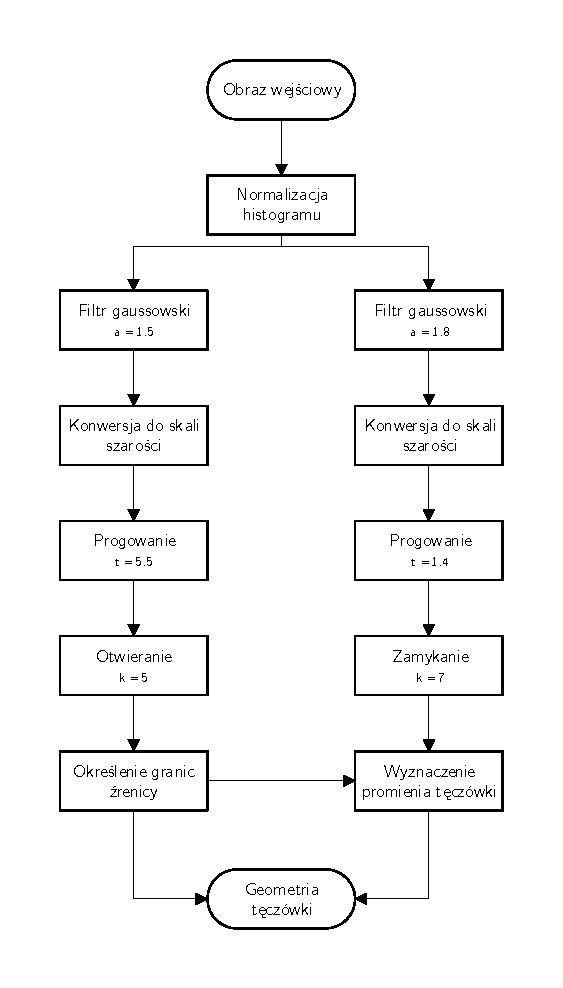
\includegraphics[height=20cm]{res/img/diagram.pdf}
    \caption{Schemat blokowy opracowanego procesu segmentacji oka.}
    \label{fig:block-diagram}
\end{figure}

\paragraph{Rozwinięcie tęczówki w~prostokąt.}
Segmentację kończy rozwinięcie tęczówki w~prostokątny obraz o~wymiarach $720 \times 400$.
Rozwinięcie to~odbywa~się poprzez przejście ze~współrzędnych polarnych na~kartezjańskie.
Dla~każdego piksela $(\theta,r)$ obrazu wynikowego wyznaczane~są współrzędne tego~punktu na~obrazie wyjściowym ze~wzorów
\begin{align*}
    \varphi &= 2 \pi \frac{\theta}{720} \\
    r' &= \frac{r}{400} (r_i - r_p) + r_p \\
    x &= r' \cos \varphi \\
    y &= r' \sin \varphi
\end{align*}
gdzie $r_i$ to~zewnętrzny promień tęczówki, a~$r_p$ --- wewnętrzny promień tęczówki (promień źrenicy).

Ponieważ wynikowe współrzędne $(x,y)$ są~ułamkowe, finalnie stosowana jest~interpolacja dwuliniowa na~kwadracie ze~wzoru
\begin{align*}
    f(x, y) = & f(\left\lfloor x \right\rfloor, \left\lfloor y \right\rfloor) \cdot (1 - \{ x \}) \cdot (1 - \{ y \}) + \\
    & f(\left\lceil x \right\rceil, \left\lfloor y \right\rfloor) \cdot \{ x \} \cdot (1 - \{ y \}) + \\
    & f(\left\lfloor x \right\rfloor, \left\lceil y \right\rceil) \cdot (1 - \{ x \}) \cdot \{ y \} + \\
    & f(\left\lceil x \right\rceil, \left\lceil y \right\rceil) \cdot \{ x \} \cdot \{ y \}
\end{align*}
gdzie $\{ x \}$ oznacza część ułamkową liczby~$x$: $\{ x \} = x - \left\lceil x \right\rceil$.

Aby zmniejszyć liczbę nieistotnych szczegółów w~rozwiniętym obrazie, przed~rozwijaniem stosowany jest filtr splotowy~Gaussa ze~współczynnikiem~1 (tj.~filtr uśredniający).

\subsection{Rozpoznawanie na~podstawie wysegmentowanej tęczówki}
\label{subsec:recognition}
Dalsza część algorytmu rozpoznawania działa na~rozwiniętym zdjęciu tęczówki.
Z~racji na~możliwość obrotu tęczówki, przy porównywaniu uwzględniane~są zdjęcia tęczówki z~obrotem co~stopień w~przedziale $[-20^\circ, 20^\circ]$.

\paragraph{Podział rozwiniętej tęczówki na~pasma.}
Zgodnie z~algorytmem zaproponowanym przez~Daugmana~\cite{slot2008}, po~rozwinięciu obraz tęczówki dzielony jest na~8 pasów o~równej szerokości w~kierunku radialnym.

Aby~uniknąć włączania rzęs lub~powiek do~analizy, pasma nie~są brane pod~uwagę w~całości.
Przyjmując, że kąty w~stopniach liczone~są od~dodatniej półosi~OY (tj. kąt~$0^\circ$ kieruje~się w~górę), brane~są pod~uwagę następujące przedziały:
\begin{itemize}
    \item dla pasm $\{ 1, 2, 3, 4 \}$ --- kąty $[0^\circ, 165^\circ] \cup [195^\circ, 360^\circ]$,
    \item dla pasm $\{ 5, 6 \}$ --- kąty $[33.5^\circ, 146.5^\circ] \cup [213.5^\circ, 326.5^\circ]$,
    \item dla pasm $\{ 7, 8 \}$ --- kąty $[45^\circ, 135^\circ] \cup [225^\circ, 315^\circ]$.
\end{itemize}

\paragraph{Zastosowanie transformaty falkowej Gabora.}
Wyznaczone pasma tęczówki są~następnie uśredniane w~kierunku radialnym, w~celu sprowadzenia ich do~postaci jednowymiarowej funkcji intensywności $I(x)$.
Uśrednianie to~jest ważone, z~użyciem funkcji~Gaussa.
Ta~funkcja jest później dyskretyzowana za~pomocą transformaty falkowej Gabora, której współczynniki wyznaczane~są ze~wzoru
$$ c_k = \sum_{i=1}^n I(x_i) \exp \left( -\frac{(x_i - x_k)^2}{\sigma^2} \right) \exp (-i 2 \pi f x_i) $$
gdzie:
\begin{itemize}
    \item $k = \{1, 2, \dots, n\}$ --- indeks próbki; w~opracowanym programie przyjęto $n = 128$,
    \item $f$ to częstotliwość falki~Gabora, która jest parametryzowana w~programie przez opcję ustawień (\keys{Settings...}),
    \item $\sigma$ to tzw. rozmycie falki; zgodnie z~\cite{slot2008} przyjmuje~się $\sigma = \frac{1}{2} \pi f$.
\end{itemize}

\paragraph{Wyznaczenie kodu tęczówki.}
Wynikowe współczynniki transformaty są~liczbami zespolonymi ($c_k \in \mathbb{C}$).
Każdy ze~współczynników konwertowany jest na~dwa bity binarne:
\begin{itemize}
    \item Pierwszy bit jest równy 1, gdy część urojona współczynnika jest ujemna ($\Im c_k < 0$) i~0 w~przeciwnym przypadku,
    \item Drugi bit jest równy 1, gdy część rzeczywista współczynnika jest ujemna ($\Re c_k < 0$) i~0 w~przeciwnym przypadku.
\end{itemize}
W~ten sposób uzyskiwane jest $128 \times 2 \times 8 = 2048$ bitów informacji, które nazywane~są kodem tęczówki.

\paragraph{Porównywanie kodów tęczówek.}
Nowe obrazy osób do~zidentyfikowania poddawane~są temu samemu procesowi przetwarzania.
W~ten sposób uzyskiwany jest zestaw kodów $c_1, \dots, c_k$ (z~różnymi kątami obrotu), który należy porównać z~zestawami kodów $c'_1, \dots, c'_k$ zawartymi w~bazie.

Porównywanie odbywa~się poprzez obliczenie wartości
$$ d = \min_{i=1,\dots,k} \min_{j=1,\dots,k} 2048 - d_H(c_i, c'_j) $$
gdzie~$d_H(x, y)$ to~odległość Hamminga między dwoma~ciągami binarnymi długości $m$:
$$ d_H(x, y) = \left| \{ i=1,\dots,m : x_i \neq y_i \} \right| $$
tj.~liczba pozycji, na~których ciągi $x, y$ różnią~się.

Im~mniejsza wartość $d$, tym~bliższe jest dopasowanie obrazu identyfikowanego do~obrazu z~bazy.
Z~tego względu jako~wynik identyfikacji brany jest~rekord z~bazy minimalizujący $d$, gdzie ta~minimalna odległość jest~miarą jakości identyfikacji, tj. jeśli jest ona zbyt~duża, rozpoznawany obraz jest~odrzucany jako~niepasujący do~żadnego rekordu w~bazie.

\section{Wyniki działania metody}
% TODO

\section{Podsumowanie}
% TODO

\begin{thebibliography}{9}

    \bibitem{daugman2004}
        Daugman J.,
        ,,How Iris Recognition Works'',
        \emph{IEEE Transactions on Circuits and Systems for Video Technology},
        tom~14,
        nr~1,
        2004.
        
    \bibitem{mmu}
        MMU Iris Dataset
        [Online].
        Dostępne: \url{http://www.cs.princeton.edu/~andyz/downloads/MMUIrisDatabase.zip}

    \bibitem{javafx}
        Oracle Corporation,
        ,,OpenJFX'',
        dokumentacja on-line.
        Dostępne: \url{https://wiki.openjdk.java.net/display/OpenJFX/Main}.

    \bibitem{slot2008}
        Ślot K.,
        \emph{Wybrane zagadnienia biometrii},
        Wydawnictwa Komunikacji i~Łączności,
        Warszawa 2008.

\end{thebibliography}

\end{document}
